\chapter{Proposed approach}

In the previous chapter, a review of two splicing detection methods based on illuminant colors analysis has been presented. However, their effectiveness still needed to be improved for real forensic applications.

The approach proposed in this chapter has been developed to correct some drawbacks and mainly to achieve an improved accuracy over the two approaches presented in Chapter 1. 

\section{Overview}

Most of the times, the splicing detection process relies on the expert's experience and background knowledge. This process usually is time consuming and error prone once that image splicing is more and more sophisticated and an aural (e.g., visual) analysis may not be enough to detect forgeries.

This approach to detecting image splicing is developed aiming at minimizing the user interaction. 

The two methods, presented in the previous chapter \cite{carvalho2016illuminant} and \cite{fan2015image}, are now being used in synergy with each other, going to analyze each image at the same time looking for potential signs of forgery.

Starting from an image we want to analyze, the method will output a set of results.
\begin{itemize}
\item A classification \textbf{label} indicating whether an image is believed to be original or counterfeit.
\item A classification \textbf{score} indicating the confidence of the method output.
\item A \textbf{detection map} highlighting the detected spliced regions.
\end{itemize}

The proposed approach minimizes human interaction being fully automated. However, not both the modules can operate in any circumstance. The face splicing detection module will work only if there is a number of faces greater than or equal to two.

\section{Face splicing detection module}

The first module is to implement, with a few enhancements and simplifications, the method proposed by Carvalho et al. \cite{carvalho2016illuminant} and presented in Section 1.6.

The algorithm to analyze an image that contains at least two sides, and whether the faces have changed or not. In particular, in the case of a fake, you can tell which of the faces in the image is false.

The method requires an initial training phase, in which you must have a dataset with faces noted. The considered dataset is the DSO-1.

This module consists of 4 consecutive stages:

\begin{enumerate}
\item \textbf{Illuminant maps extraction}: given an input image, two different illuminant maps are evaluated, using the IIC and GGE extraction methods.
\item \textbf{Face detection}: after the illuminant maps extraction, the human faces in the image are detected. In the training phase the faces positions are read from the groundtruth file. If the given image contains less than two faces, it is discarded.
\item \textbf{Paired face feature extraction}: human faces are considered and classified in pairs. From each extracted face in the previous step, a color descriptor is used in order to extract features.
\item \textbf{KNN models training}: fixed a value of $K$, a set of KNN models are trained using previous feature vectors.
\item \textbf{Forgery detection and classification}: in this step an image is classified as fake or normal. Given an image classified as fake, the analysis is refined pointing out which part of the image is the result of a composition.
\end{enumerate}

\subsection{Illuminant maps extraction}

Given a single image $I$ the two different illuminant maps are extracted: both generalized grayworld algorithm (GGE) and inverse-intensity chromaticity estimation (IIC) are used.

\begin{figure}[!htb]
\minipage{0.32\textwidth}
  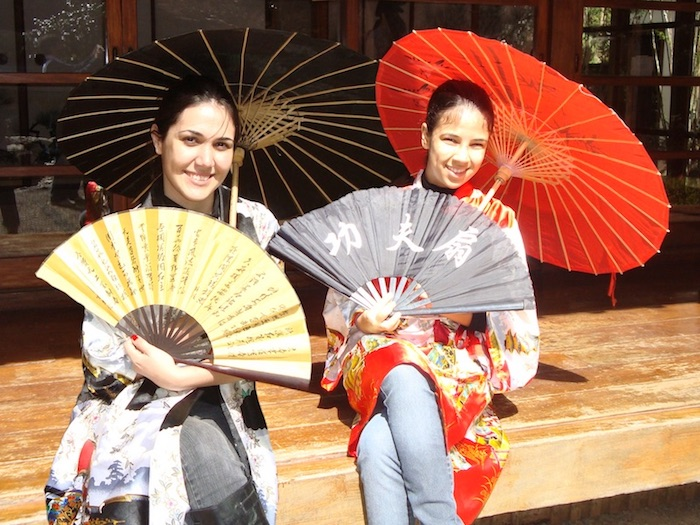
\includegraphics[width=\linewidth]{splicing-33.jpg}
  \caption{The original image}\label{fig:awesome_image1}
\endminipage\hfill
\minipage{0.32\textwidth}
  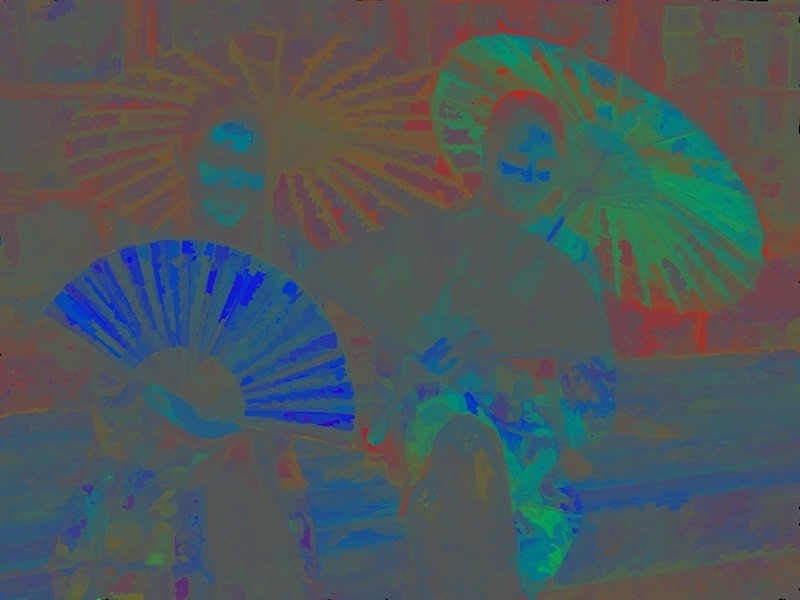
\includegraphics[width=\linewidth]{splicing-33_gge_map.jpg}
  \caption{GGE illuminant map}\label{fig:awesome_image2}
\endminipage\hfill
\minipage{0.32\textwidth}%
  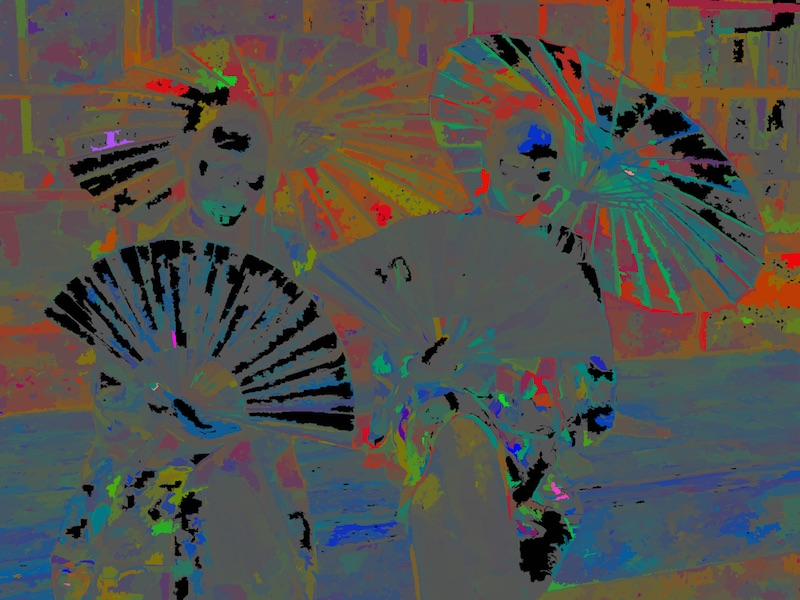
\includegraphics[width=\linewidth]{splicing-33_iic_map.jpg}
  \caption{IIC illuminant map}\label{fig:awesome_image3}
\endminipage
\end{figure}

Differently from de Carvalho et al. \cite{carvalho2016illuminant}, who have used the conversion of IMs to the YCbCr color space, the two IMs are considered as two different color maps theirself.

\subsection{Face detection}

One of the major drawback of the method proposed by Carvalho et al. \cite{carvalho2016illuminant} relies on the user interaction needed for detecting human faces in the image. In this approach a common face detection module is used to achieve the same results, aiming at minimizing the user dependency and making the entire algorithm user independent.

The face detector used is the one initially proposed by Viola and Jones \cite{viola2001rapid}\cite{viola2004robust} and improved by  Lienhart et al. \cite{lienhart2002extended}. Usually called simply Viola-Jones, its original motivation was face detection, but it can be trained to detect different object classes. 

This detector combines four key concepts: 
\begin{itemize}
\item Simple rectangular features, called \emph{Haar features}
\item \emph{Integral Image}\cite{crow1984summed} concept for rapid feature detection 
\item \emph{AdaBoost}\cite{freund1995desicion} machine-learning method 
\item A \emph{cascade classifier} to combine all features efficiently 
\end{itemize}

The used rectangle combinations are not true \emph{Haar wavelets}\cite{haar1910theorie}. Instead, they contain better suited rectangle combinations used for visual object detection. The presence of a Haar feature is determined by subtracting the pixel values of the dark region to the pixel values of the light one. If the difference exceeds some threshold value set during the training process, the feature is said to be present. 

\begin{figure}[h!]
  \centering
    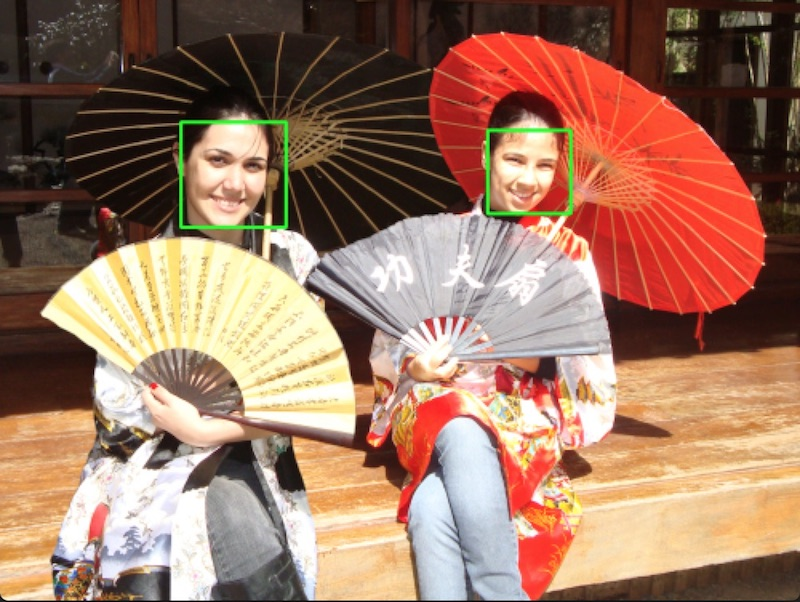
\includegraphics[width=0.5\textwidth]{facedetected}
    \caption{The output of the face detection module}
    \label{fig:facesdetected}
\end{figure}

\emph{OpenCV}\footnote{OpenCV - Open source computer vision. http://opencv.org} provides an implementation of the Viola-Jones face detector as \emph{cvHaarDetectObjects}.

Figure \ref{fig:facesdetected} shows the output of the face detector module. Given the faces bounding boxes, the corresponding regions in the illuminant maps are extracted, figure \ref{fig:facesdetectedmaps}.

\begin{figure}[h!]
  \centering
    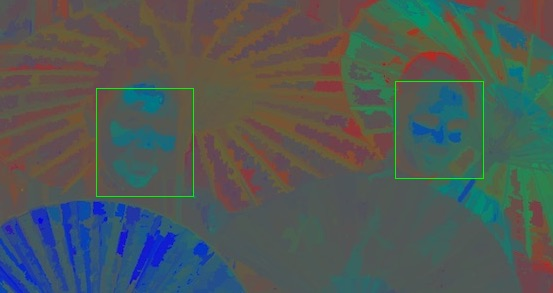
\includegraphics[width=0.5\textwidth]{splicing-33_gge_map_faces}
    \caption{The extracted faces from illuminant map}
    \label{fig:facesdetectedmaps}
\end{figure}

\subsection{Paired face feature extraction}

From each extracted face in the previous step, we need to find telltales that allow identification of spliced images. 

According to Riess and Angelopoulou \cite{riess2010scene}, when the output illumination maps are analyzed by an expert for detecting forgeries, the main observed feature is color. Thus, differently from Carvalho et al. \cite{carvalho2016illuminant} who have explored a large set of descriptors of different visual properties (e.g., texture, shape, color, among others) we focused our attention on color descriptors.

The considered color description techniques are ACC \cite{huang1997image}, BIC \cite{stehling2002compact}, CCV \cite{pass1997comparing}, and LCH \cite{swain1991color}.

\subsubsection{ACC descriptor}

\emph{Color Autocorrelogram (ACC) }\cite{huang1997image} maps the spatial information of colors by pixels correlations in different distances. Let $I$ an image, the \emph{autocorrelogram} (the term \emph{“correlogram”} is adapted from spatial data analysis \cite{upton1985spatial}) computes the probability of finding two pixels in $I$ with a color $c$ in a distance $d$ from each other. 

After the autocorrelogram computation, a set of $m$  probability values for each distance $d$ are considered, where $m$ stands for the number of colors in the quantized space. 

The implemented version quantized the RGB color space into 64 bins and considered 4 distance values (1, 3, 5, and 7). The \emph{L1} distance function is used.

\subsubsection{BIC descriptor}

\emph{Border/Interior Pixel Classification (BIC)} \cite{stehling2002compact} is a region-based color descriptor. Its extraction algorithm classifies the image pixels in border or interior
pixels. 

The image is first quantized into 64 colors in RGB color space. Then, each pixel is classified as interior
if its neighbors (above, below, left and right pixels) have the same color. Otherwise it is classified as border pixel. After the classification, two histograms are generated: one for border pixels and other for interior pixels. These histograms are stored as one single histogram with 128 bins. The distance
function is called \emph{dLog} and it compares histograms in a logarithmic scale. 

\subsubsection{CCV descriptor}

\emph{Color Coherence Vector (CCV)} \cite{pass1997comparing} is a very popular color descriptor in the literature. Its extraction algorithm classifies the image pixels in coherent or incoherent pixels. This classification considers if the pixel belongs or not to a region with similar colors, called \emph{coherent region}. After the classification, two color histograms are computed: one for coherent pixels and other for incoherent pixels.

Both histograms are concatenated to compose the final feature vector. The RGB color space is quantized into 64 bins and L1 distance function is used.

\subsubsection{LCH descriptor}

\emph{Local Color Histogram (LCH)} \cite{swain1991color} is one of the most popular descriptors that is based on fixed size regions to describe image properties. Its extraction algorithm splits the image into fixed size blocks and computes a color histogram for each region. After that, the histograms of each region
are concatenated to compose one single histogram. 

The implemented version splits the image
in 16 regions (4x4 grid) and quantized the RGB color space into 64 bins. This generated feature vectors with 1024 values. The L1 distance function is used.


\subsubsection{Paired features}

In order to detect a face forgery, we need to compare  the current analyzed image region against other, looking for color inconsistencies. Thus, instead of considering each face separately, a paired face feature vector is encoded for every possible face pair.

Given two face descriptors, $\mathcal{D_1}$ and $\mathcal{D_2}$, whose length depends on the color descriptor used, the final descriptor is computed concatenating them into a single feature vector $\mathcal{P}$. So, in an image $I$ containing $q$ faces, a set $S$ of feature vectors are extracted, with

$$
S = \{\mathcal{P}_1, \ldots, \mathcal{P}_m\} \quad \textrm{  where } m = \frac{q (q-1)}{2}
$$

if $q \geq 2$. 

Each face descriptor is computed twice, one based on the GGE map and one based on the IIC map.

\subsection{KNN models training}

After the feature vectors are extracted from all faces in the images, a set of 8 \emph{k-nearest neighbors} classifiers are trained algorithm, 4 models based on the GGE map and 4 based on the IIC map. 

These models will be used in the classification step with majority voting.

\subsection{Forgery detection and classification}

Differently from Carvalho \emph{et al.} \cite{carvalho2016illuminant}, we used a different approach for classifying the single face as fake using the results of the paired face classification. 

Let $P_{i, j}$ the paired feature vector computed concatenating the $i$-th and the $j$-th face feature. If $P_{i, j}$ is classified as fake, the scores of the considered images are incremented by one unit. At the end of the process, faces with a higher associated scores have been classified as fake multiple times.

The resulting scores are then thresholded for selecting the most probably doctored faces. 

Given an input image $I$ containing $q$ faces, the forgery detection algorithm is summarized in Algorithm \ref{alg:faceforgerydetection}.

\begin{algorithm}[!h]
\begin{algorithmic}[1]
\For {$im \in \{GGE, IIC\}$}
\For {$desc \in \{ACC, BIC, CCV, LCH\}$}
\State $F = extractFeatures(im, desc)$
\State So $F = \{\mathcal{P}_1, \ldots, \mathcal{P}_m\} $ where $ m = \frac{q(q-1)}{2}$
\For {$f in F$}
\State $prediction = KNN.predict(f)$
\If {$prediction = Positive$}
\State Let $i, j$ the faces considered for $f$ evaluation
\State Increment $i, j$ scores
\EndIf
\EndFor
\EndFor
\EndFor
\end{algorithmic}\caption{Face forgery detection}\label{alg:faceforgerydetection}
\end{algorithm}

The output of the detector is a resulting detection mask, which highlights the spliced part of the image.

\begin{figure}[h!]
  \centering
    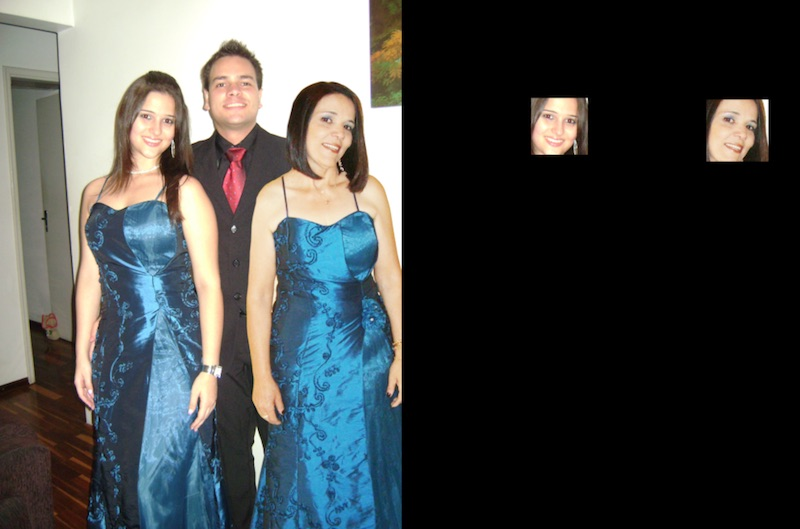
\includegraphics[width=0.55\textwidth]{facesplicingdetectionoutput}
    \caption{The output splicing detection module}
    \label{fig:facesplicingdetectionoutput}
\end{figure}

An example is shown in Figure \ref{fig:facesplicingdetectionoutput}. The two women in the image are counterfeited and their faces are shown in the resulting detection map as fake. In this particular case the detector has a perfect accuracy. 

\section{Region splicing detection module}

The second form of the algorithm is to implement the method proposed by Fan et al.\cite{fan2015image} with some changes in order to try to correct some of its major drawbacks presented in Section 1.7.

The splicing detection task performed by our approach consists in labelling a new image among two pre-defined classes (real and fake) and later pointing the face with higher probability to be the fake face. In this process, a classification model is created to indicate the class to which a new image belongs.

In summary, this module consists of the 6 main steps:

\begin{itemize}
\item \textbf{Image segementation}: relies on vertical and horizontal image segmentations. The outputs of this stage are two set of directional image bands. 
\item \textbf{Band illuminant estimation}: consists in estimating the illuminant color for each segmented band using 5 different GGE algorithms.
\item \textbf{Reference illuminant estimation}: consists in estimating the illuminant reference value for each direction.
\item \textbf{Feature vector evaluation}: relies on encoding the singular band illuminant information into a feature vector for further classification. The feature vector elements are the differences between the current illuminant color and the reference one.
\item \textbf{Band classification}: consists in labelling each image band into one of the know classes (real or fake) based on the previously learned classification model.
\item \textbf{Detection map}: using the classification output of the previous step, a detection map is build. The higher the value of this map, the higher the  resulting classification score for a single pixel.
\end{itemize}

\begin{figure}[h!]
  \centering
    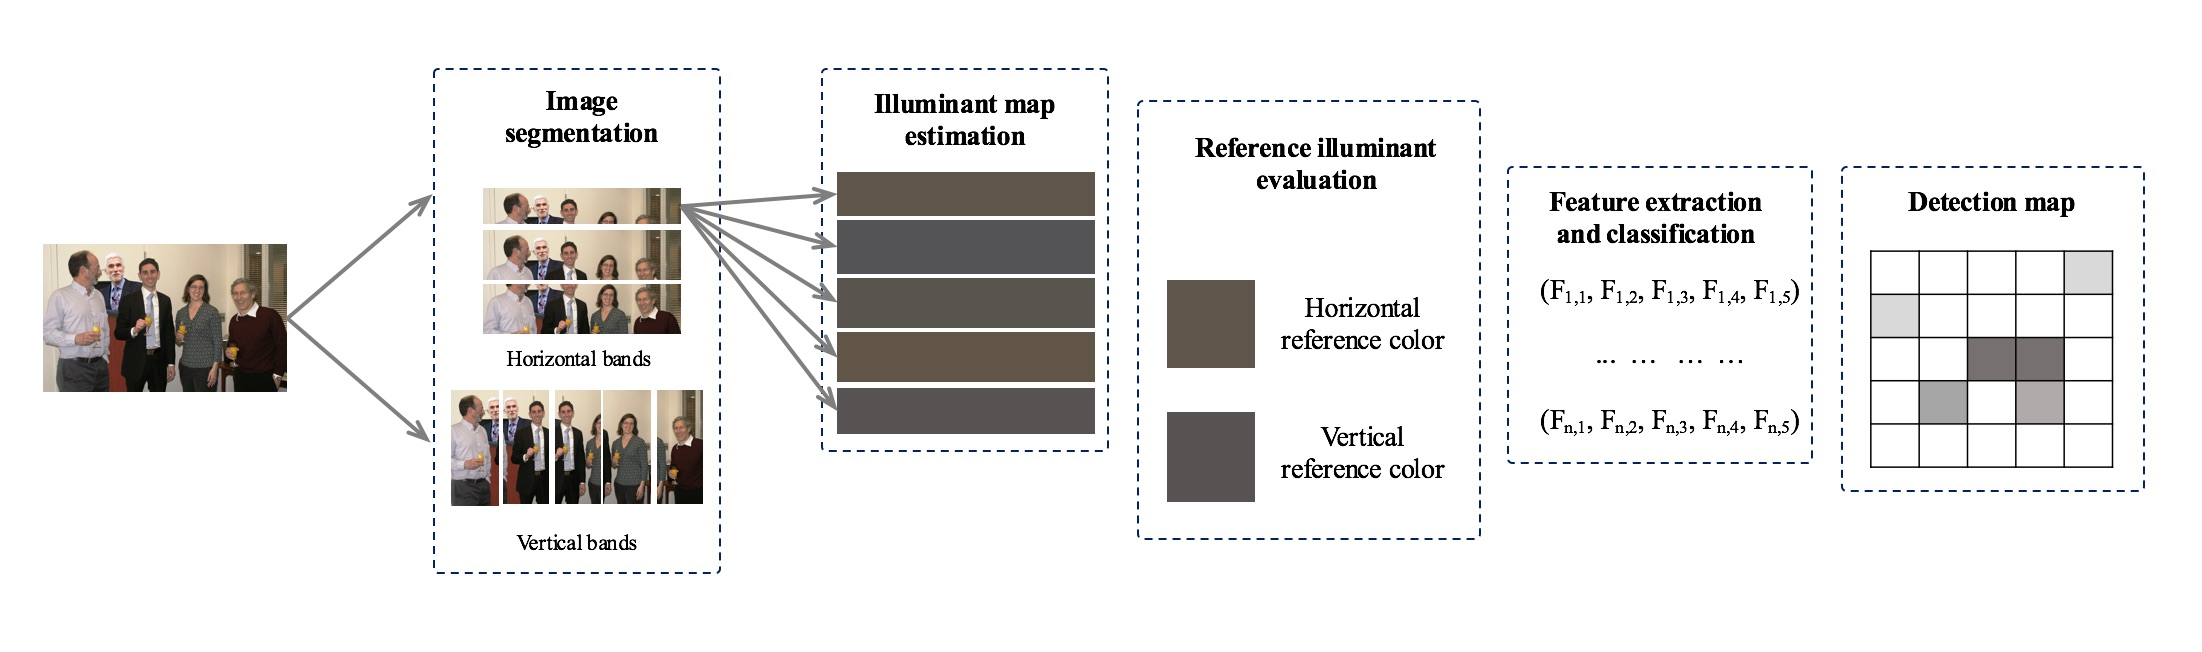
\includegraphics[width=1\textwidth]{pipeline_regions}
    \caption{Image regional splicing detection module pipeline}
    \label{fig:regionsmodulepipeline}
\end{figure}

The Fig \ref{fig:regionsmodulepipeline} summarize the module pipeline.

\subsection{Image segmentation}

In the first step of the process, the input image is segmented in order to obtain two image bands categories: horizontal and vertical bands. This kind of segmentation method is chosen because of its simplicity.

First, a band width $B_w$ and a band height $B_h$ is set. Due to the fact that the segmentation has to produce overlapping bands, we set a delta factor of $\frac{1}{4}$. As a result we get overlapping stripes for a total of 25\% of their area. 

The choice of the band size is a crucial phase of the algorithm: a band too tight would fail to capture the information necessary to classify our object of interest as falsified, unlike a band too wide would capture instead too much additional information.

The choice of the overlapped area percentage makes possible a more detailed evaluation. In this way it is possible to classify the same region of the image more than once, increasing the expressive power of our final classifier, the detection map.
 
In summary, let $I$ be the input image. After the segmentation process we obtain a set $B$ of bands containing all vertical and horizontal bands:

$$
B = \{V_1, \ldots, V_n, H_1, \ldots, H_m\}
$$

The dimension of $B$ is given by the sum of the number of vertical ($n$) and horizontal ($m$) bands.

\subsection{Band illuminant estimation}

The resulting image bands are now processed in order to evaluate the illuminant color using different techniques.

For this step, the Generalized Grayworld \cite{van2007edge} algorithms are used, as presented in Chapter 1. For each band, the illumination estimation is accomplished by using one of algorithms composed of Grey-World, Max-RGB, Shades of Grey, first-order Grey-Edge and second-order Grey-Edge. Thus we have 5 illuminant estimates for each band.
Table \ref{table:ggemethods} in Chapter 1 summarize this algorithm parameters.

In this way we obtain 5 different illuminant estimation for each single band.

$$
\forall b \in B \qquad R_a(b) = GGE_a(b) \qquad a \in \mathcal{A}
$$

where $\mathcal{A}$ is the set of the previously mentioned algorithms and $GGE$ is the algorithm implementation.

\subsection{Reference illuminant estimation}

After estimating the illuminant of each horizontal/vertical band, it is evaluated a reference illuminant color for each used algorithms.

$$
\forall a \in \mathcal{A} \qquad RV_a = median(R_a(b)) \quad \forall \; b \textrm{ vertical}
$$
$$
\forall a \in \mathcal{A} \qquad RH_a = median(R_a(b)) \quad \forall \; b \textrm{ horizontal}
$$

where $RV_a$ and $RH_a$ are the reference illuminant colors for the $a$ algorithm for vertical and horizontal direction respectively. As these two values are calculated using the median, will be identical to one of the values of a band of that same direction.

\subsection{Feature vector estimation}

Given the two reference color for each of the two directions, a feature band for each single image band can be built.

Assuming a single light source in the image, all the evaluated illuminant will point at the same color.
Based on this assumption, a feature vector that capture how the gang present of singularities in the illuminant is built.

Let $b \in B$ a single band lying on $d \in \{vertical, horizontal\}$ direction. The feature vector for $b$ will be:

\begin{equation}\label{eq:regionsfeaturevector}
f_{b} = \{m_1, m_2, m_3, m_4, m_5\}
\end{equation}
where
$$
m_i = dist(R_a(b) - RC)
$$
where $RC = RV_a$ or $RC = RH_a$ in case of vertical and horizontal band respectively and $dist$ is the Euclidean distance function between two RGB values.

\subsection{Band classification}

Given a feature vector, a machine learning approach is used to automatically classify the band. 
In a prior step, a classification model is trained using a set of sample data. A Support Vector Machine (SVM) classifier with a radial basis function (RBF) kernel is used.

$$
\forall \; b \in B \quad Label(b) = SVM(b)
$$

\subsection{Detection map}

In order to collect all the classification outputs, a detection map is build and updated after each evaluation. If the result of the classification is \emph{positive} (\emph{fake}), all the pixel values that belong to the band portion in the image will be increased by one unit.

At the end of the process, all the splicing region pixels will have greater values than the others. At this stage a color map is displayed to give a visual feedback for locating the splicing image parts.


